%%%%%%%%%%%%%%%%%%%%%%%%%%%%%%%%%%%%%%%%%
% Beamer Presentation
% LaTeX Template
% Version 1.0 (10/11/12)
%
% This template has been downloaded from:
% http://www.LaTeXTemplates.com
%
% License:
% CC BY-NC-SA 3.0 (http://creativecommons.org/licenses/by-nc-sa/3.0/)
%
%%%%%%%%%%%%%%%%%%%%%%%%%%%%%%%%%%%%%%%%%

%----------------------------------------------------------------------------------------
%	PACKAGES AND THEMES
%----------------------------------------------------------------------------------------

\documentclass{beamer}

\mode<presentation> {

% The Beamer class comes with a number of default slide themes
% which change the colors and layouts of slides. Below this is a list
% of all the themes, uncomment each in turn to see what they look like.

%\usetheme{default}
%\usetheme{AnnArbor}
%\usetheme{Antibes}
%\usetheme{Bergen}
%\usetheme{Berkeley}
%\usetheme{Berlin}
%\usetheme{Boadilla}
%\usetheme{CambridgeUS}
%\usetheme{Copenhagen}
%\usetheme{Darmstadt}
%\usetheme{Dresden}
%\usetheme{Frankfurt}
%\usetheme{Goettingen}
%\usetheme{Hannover}
%\usetheme{Ilmenau}
%\usetheme{JuanLesPins}
%\usetheme{Luebeck}
%\usetheme{Madrid}
%\usetheme{Malmoe}
%\usetheme{Marburg}
%\usetheme{Montpellier}
\usetheme{PaloAlto}
%\usetheme{Pittsburgh}
%\usetheme{Rochester}
%\usetheme{Singapore}
%\usetheme{Szeged}
%\usetheme{Warsaw}

% As well as themes, the Beamer class has a number of color themes
% for any slide theme. Uncomment each of these in turn to see how it
% changes the colors of your current slide theme.

%\usecolortheme{albatross}
%\usecolortheme{beaver}
%\usecolortheme{beetle}
%\usecolortheme{crane}
%\usecolortheme{dolphin}
%\usecolortheme{dove}
%\usecolortheme{fly}
%\usecolortheme{lily}
%\usecolortheme{orchid}
%\usecolortheme{rose}
%\usecolortheme{seagull}
%\usecolortheme{seahorse}
%\usecolortheme{whale}
%\usecolortheme{wolverine}

%\setbeamertemplate{footline} % To remove the footer line in all slides uncomment this line
%\setbeamertemplate{footline}[page number] % To replace the footer line in all slides with a simple slide count uncomment this line

%\setbeamertemplate{navigation symbols}{} % To remove the navigation symbols from the bottom of all slides uncomment this line
}

\usepackage{graphicx} % Allows including images
\usepackage{booktabs} % Allows the use of \toprule, \midrule and \bottomrule in tables

%----------------------------------------------------------------------------------------
%	TITLE PAGE
%----------------------------------------------------------------------------------------

\title[Practica 1]{Practica 1: Eficiencia} % The short title appears at the bottom of every slide, the full title is only on the title page

\author{Algoritmica} % Your name
\institute[UGR] % Your institution as it will appear on the bottom of every slide, may be shorthand to save space
{
Universidad de Granada \\ % Your institution for the title page
\medskip

}
\date{\today} % Date, can be changed to a custom date

\begin{document}

\begin{frame}
\titlepage % Print the title page as the first slide
\end{frame}

\begin{frame}
\frametitle{Indice} % Table of contents slide, comment this block out to remove it
\tableofcontents % Throughout your presentation, if you choose to use \section{} and \subsection{} commands, these will automatically be printed on this slide as an overview of your presentation
\end{frame}

%----------------------------------------------------------------------------------------
%	PRESENTATION SLIDES
%----------------------------------------------------------------------------------------

\section{Introduccion }
\begin{frame}
	\frametitle{Introduccion}
	\begin{itemize}
		\item El objetivo de ésta práctica era analizar eficiencias de forma empírica e híbrida.
		\item Para ello, hemos recogido los diferentes tiempos de los diferentes algoritmos que se ofrecían y los hemos comparado.
		\item En nuestro caso concreto, hemos utilizado la biblioteca de C++ más moderna y precisa destinado a obtener tiempos de reloj: la biblioteca \textbf{chrono}
	
	\end{itemize}
\end{frame}


%------------------------------------------------
\section{Ordenacion} % Sections can be created in order to organize your presentation into discrete blocks, all sections and subsections are automatically printed in the table of contents as an overview of the talk
%------------------------------------------------
\begin{frame}
	\frametitle{Ordenación}
	Según hemos ido hemos estudiado, estos algoritmos que presentamos tienen teóricamente y calculando a partir del código una eficiencia de O(n ^2 ). Como esto es teórico, vamos a ver si efectivamente (o no) los algoritmos proporcionados se parecen a la grafica de n² recogiendo la informacion de 99 posibilidades distintas en cada algoritmo.
	\begin{figure}
		\centering
		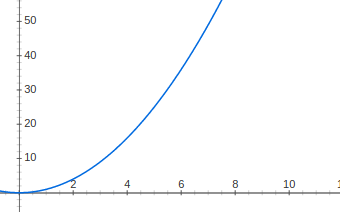
\includegraphics[width=0.7\linewidth]{imagenes/n^2}
		\caption{}
		\label{fig:E1}
	\end{figure}

\end{frame}

\subsection{Burbuja}
\begin{frame}
	\frametitle{Burbuja}
	La gráfica empírica obtenida ha sido:
	\begin{figure}
		\centering
		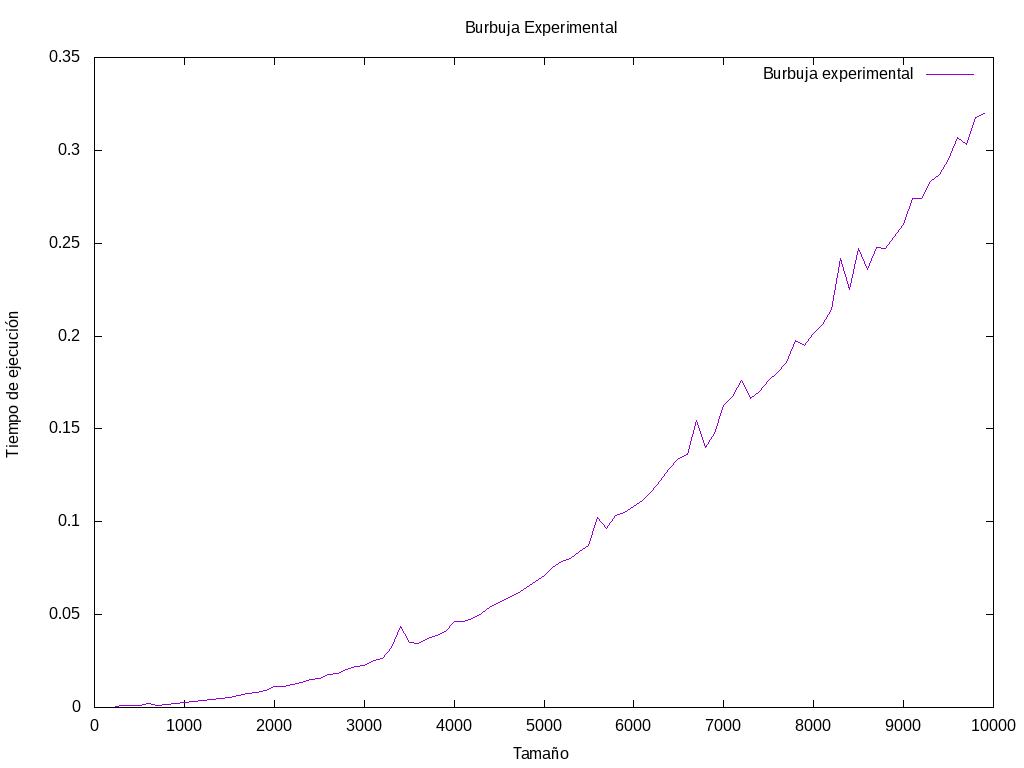
\includegraphics[width=0.7\linewidth]{imagenes/burbuja-experimental.png}
		\caption{}
		\label{fig:E2}
	\end{figure}
	
\end{frame}

\begin{frame}
	\frametitle{Burbuja}
	La gráfica híbrida obtenida ha sido:
	\begin{figure}
		\centering
		\includegraphics[width=0.7\linewidth]{imagenes/burbuja-híbrida}
		\caption{}
		\label{fig:E3}
	\end{figure}	
\end{frame}





\subsection{Seleccion}
\begin{frame}
	\frametitle{Selección}
	La gráfica empírica obtenida ha sido:
	\begin{figure}
		\centering
		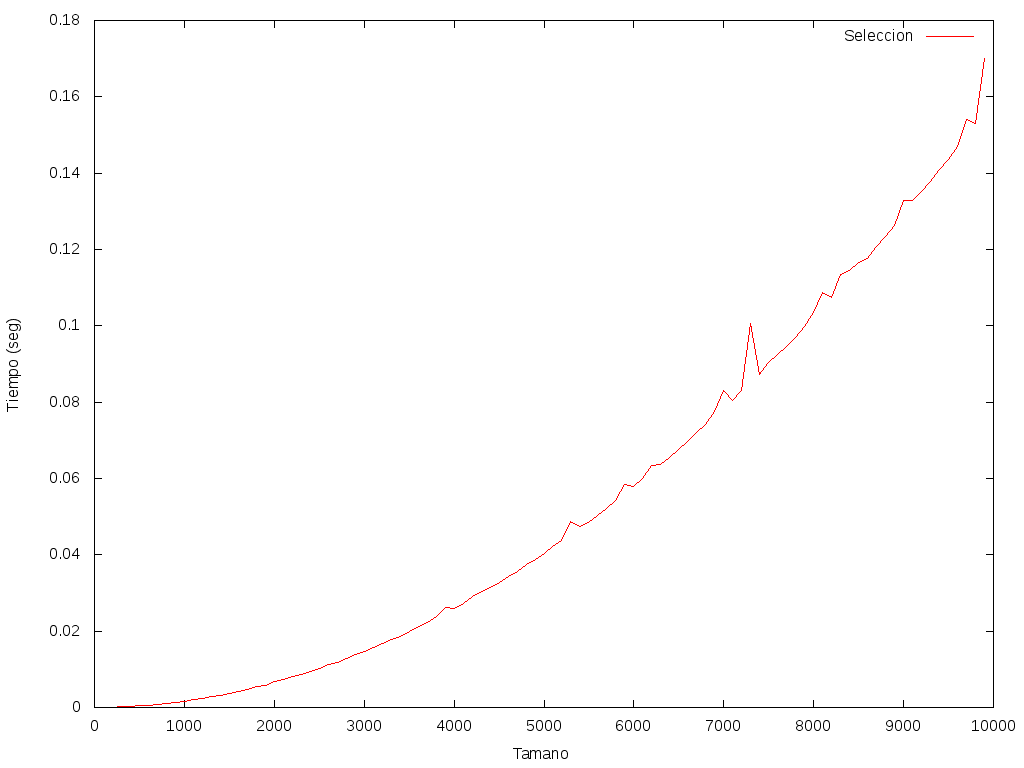
\includegraphics[width=0.7\linewidth]{imagenes/seleccionLines.png}
		\caption{}
		\label{fig:E4}
	\end{figure}
	
\end{frame}

\begin{frame}
	\frametitle{Selección}
	La gráfica híbrida obtenida ha sido:
	\begin{figure}
		\centering
		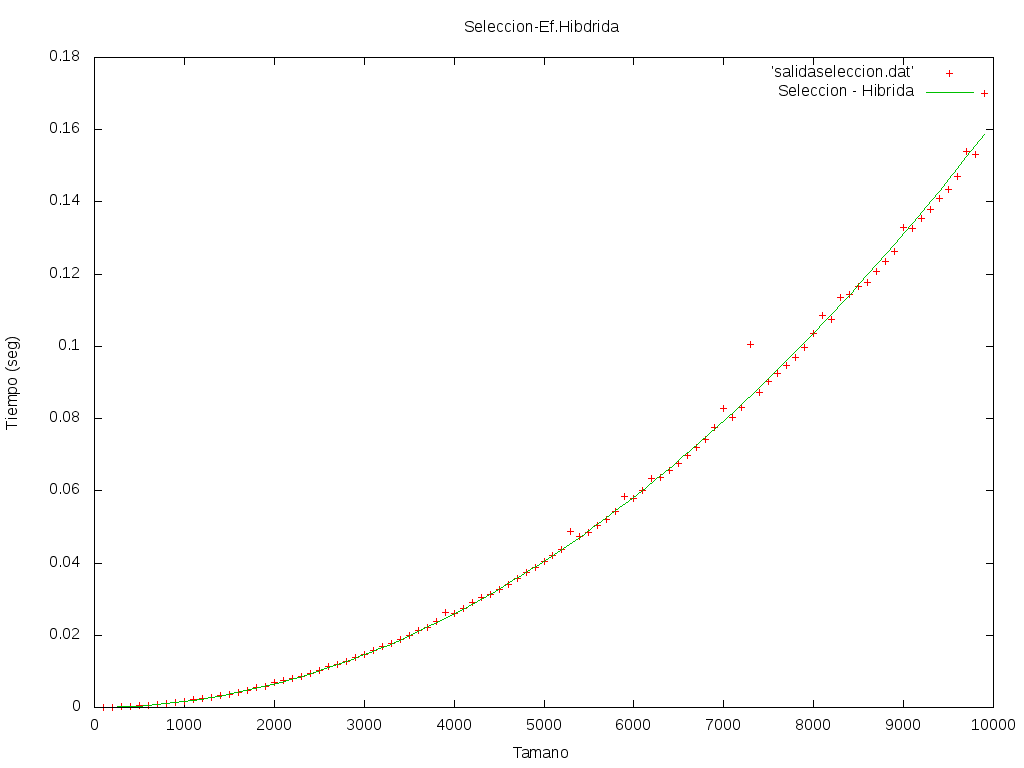
\includegraphics[width=0.7\linewidth]{imagenes/seleccion-hibrida.png}
		\caption{}
		\label{fig:E5}
	\end{figure}
	
\end{frame}
\subsection{Insercion}
\begin{frame}
	\frametitle{Inserción}
	La gráfica empírica obtenida ha sido:
	\begin{figure}
		\centering
		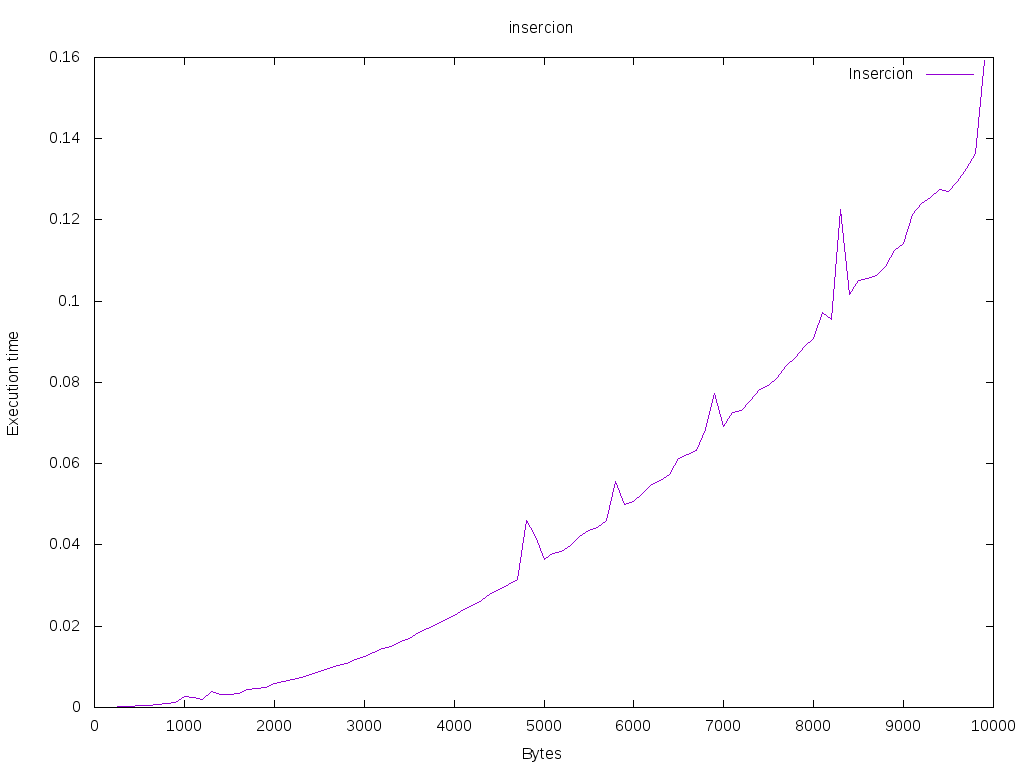
\includegraphics[width=0.7\linewidth]{imagenes/insercion.png}
		\caption{}
		\label{fig:E2}
	\end{figure}
	
\end{frame}

\begin{frame}
	\frametitle{Inserción}
	La gráfica híbrida obtenida ha sido:
	\begin{figure}
		\centering
		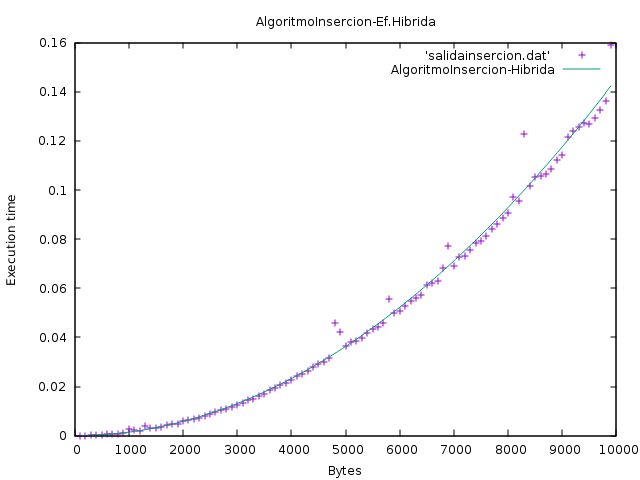
\includegraphics[width=0.7\linewidth]{imagenes/algoritmoInsercion-hibrida}
		\caption{}
		\label{fig:E3}
	\end{figure}
	
\end{frame}


\begin{frame}
	\frametitle{Inserción}
	Por ultimo, mostramos el porcentaje de error a la hora de obtener las constantes ocultas es muy bajo.
	
	
	
\end{frame}


\section{Ordenacion rapida} % Sections can be created in order to organize your presentation into discrete blocks, all sections and subsections are automatically printed in the table of contents as an overview of the talk
%------------------------------------------------

\subsection{Quick Sort}
\subsection{Heap Sort}
\subsection{Merge Sort}

\section{Floyd}
\section{Hanoi}



%------------------------------------------------

\begin{frame}
\frametitle{Bullet Points}
\begin{itemize}
\item Lorem ipsum dolor sit amet, consectetur adipiscing elit
\item Aliquam blandit faucibus nisi, sit amet dapibus enim tempus eu
\item Nulla commodo, erat quis gravida posuere, elit lacus lobortis est, quis porttitor odio mauris at libero
\item Nam cursus est eget velit posuere pellentesque
\item Vestibulum faucibus velit a augue condimentum quis convallis nulla gravida
\end{itemize}
\end{frame}

%------------------------------------------------

\begin{frame}
\frametitle{Blocks of Highlighted Text}
\begin{block}{Block 1}
Lorem ipsum dolor sit amet, consectetur adipiscing elit. Integer lectus nisl, ultricies in feugiat rutrum, porttitor sit amet augue. Aliquam ut tortor mauris. Sed volutpat ante purus, quis accumsan dolor.
\end{block}

\begin{block}{Block 2}
Pellentesque sed tellus purus. Class aptent taciti sociosqu ad litora torquent per conubia nostra, per inceptos himenaeos. Vestibulum quis magna at risus dictum tempor eu vitae velit.
\end{block}

\begin{block}{Block 3}
Suspendisse tincidunt sagittis gravida. Curabitur condimentum, enim sed venenatis rutrum, ipsum neque consectetur orci, sed blandit justo nisi ac lacus.
\end{block}
\end{frame}

%------------------------------------------------

\begin{frame}
\frametitle{Multiple Columns}
\begin{columns}[c] % The "c" option specifies centered vertical alignment while the "t" option is used for top vertical alignment

\column{.45\textwidth} % Left column and width
\textbf{Heading}
\begin{enumerate}
\item Statement
\item Explanation
\item Example
\end{enumerate}

\column{.5\textwidth} % Right column and width
Lorem ipsum dolor sit amet, consectetur adipiscing elit. Integer lectus nisl, ultricies in feugiat rutrum, porttitor sit amet augue. Aliquam ut tortor mauris. Sed volutpat ante purus, quis accumsan dolor.

\end{columns}
\end{frame}

%------------------------------------------------
\section{Second Section}
%------------------------------------------------

\begin{frame}
\frametitle{Table}
\begin{table}
\begin{tabular}{l l l}
\toprule
\textbf{Treatments} & \textbf{Response 1} & \textbf{Response 2}\\
\midrule
Treatment 1 & 0.0003262 & 0.562 \\
Treatment 2 & 0.0015681 & 0.910 \\
Treatment 3 & 0.0009271 & 0.296 \\
\bottomrule
\end{tabular}
\caption{Table caption}
\end{table}
\end{frame}

%------------------------------------------------

\begin{frame}
\frametitle{Theorem}
\begin{theorem}[Mass--energy equivalence]
$E = mc^2$
\end{theorem}
\end{frame}

%------------------------------------------------

\begin{frame}[fragile] % Need to use the fragile option when verbatim is used in the slide
\frametitle{Verbatim}
\begin{example}[Theorem Slide Code]
\begin{verbatim}
\begin{frame}
\frametitle{Theorem}
\begin{theorem}[Mass--energy equivalence]
$E = mc^2$
\end{theorem}
\end{frame}\end{verbatim}
\end{example}
\end{frame}

%------------------------------------------------

\begin{frame}
\frametitle{Figure}
Uncomment the code on this slide to include your own image from the same directory as the template .TeX file.
%\begin{figure}
%\includegraphics[width=0.8\linewidth]{test}
%\end{figure}
\end{frame}

%------------------------------------------------

\begin{frame}[fragile] % Need to use the fragile option when verbatim is used in the slide
\frametitle{Citation}
An example of the \verb|\cite| command to cite within the presentation:\\~

This statement requires citation \cite{p1}.
\end{frame}

%------------------------------------------------

\begin{frame}
\frametitle{References}
\footnotesize{
\begin{thebibliography}{99} % Beamer does not support BibTeX so references must be inserted manually as below
\bibitem[Smith, 2012]{p1} John Smith (2012)
\newblock Title of the publication
\newblock \emph{Journal Name} 12(3), 45 -- 678.
\end{thebibliography}
}
\end{frame}

%------------------------------------------------

\begin{frame}
\Huge{\centerline{The End}}
\end{frame}

%----------------------------------------------------------------------------------------

\end{document} 